\documentclass{beamer}
\usetheme{Madrid}
\usecolortheme{default}
\usepackage[utf8]{inputenc}
\usepackage[brazil]{babel}
\usepackage{graphicx}
\usepackage{booktabs}

\title[Análise de Algoritmos de Ordenação]{Análise Empírica e Comparativa de Desempenho de Algoritmos de Ordenação}
\subtitle{Ciência da Computação -- Universidade Federal do Tocantins (UFT)}
\author{Acadêmicos do Curso}
\date{\today}

\begin{document}

\frame{\titlepage}

\begin{frame}{Roteiro da Apresentação}
    \tableofcontents
\end{frame}

\section{Introdução e Objetivos}
\begin{frame}{Introdução e Objetivos}
    \begin{itemize}
        \item \textbf{Objetivo Central:} Investigar empíricamente o comportamento de 6 algoritmos de ordenação sob diferentes cenários de entrada.
        \item \textbf{Algoritmos Analisados:}
            \begin{itemize}
                \item \textbf{Quadráticos $O(n^2)$:} Bubble Sort, Selection Sort, Insertion Sort
                \item \textbf{Log-Lineares $O(n \log n)$:} Merge Sort, Quick Sort (Mediana de 3), Heap Sort
            \end{itemize}
        \item \textbf{Métricas Coletadas:} Tempo de execução, Comparações, Trocas/Movimentações.
    \end{itemize}
\end{frame}

\section{Complexidade Assintótica}
\begin{frame}{Quadro Comparativo Teórico}
    \begin{table}[H]
    \centering
    \tiny
    \begin{tabular}{@{}lcccccl@{}}
    \toprule
    \textbf{Algoritmo} & \textbf{Melhor} & \textbf{Médio} & \textbf{Pior} & \textbf{Espaço} & \textbf{Estável?} & \textbf{Estratégia} \\ \midrule
    Bubble Sort & $O(n)$ & $O(n^2)$ & $O(n^2)$ & $O(1)$ & Sim & Trocas adjacentes \\
    Selection Sort & $O(n^2)$ & $O(n^2)$ & $O(n^2)$ & $O(1)$ & Não & Mínimo iterativo \\
    Insertion Sort & $O(n)$ & $O(n^2)$ & $O(n^2)$ & $O(1)$ & Sim & Inserção direta \\
    Merge Sort & $O(n \log n)$ & $O(n \log n)$ & $O(n \log n)$ & $O(n)$ & Sim & Divisão e Conquista \\
    Quick Sort & $O(n \log n)$ & $O(n \log n)$ & $O(n^2)$ & $O(\log n)$ & Não & Particionamento \\
    Heap Sort & $O(n \log n)$ & $O(n \log n)$ & $O(n \log n)$ & $O(1)$ & Não & Heap Binário Máx \\ \bottomrule
    \end{tabular}
    \end{table}
\end{frame}

\section{Resultados Experimentais}
\begin{frame}{Tempo de Execução -- Entrada Aleatória}
    \begin{center}
        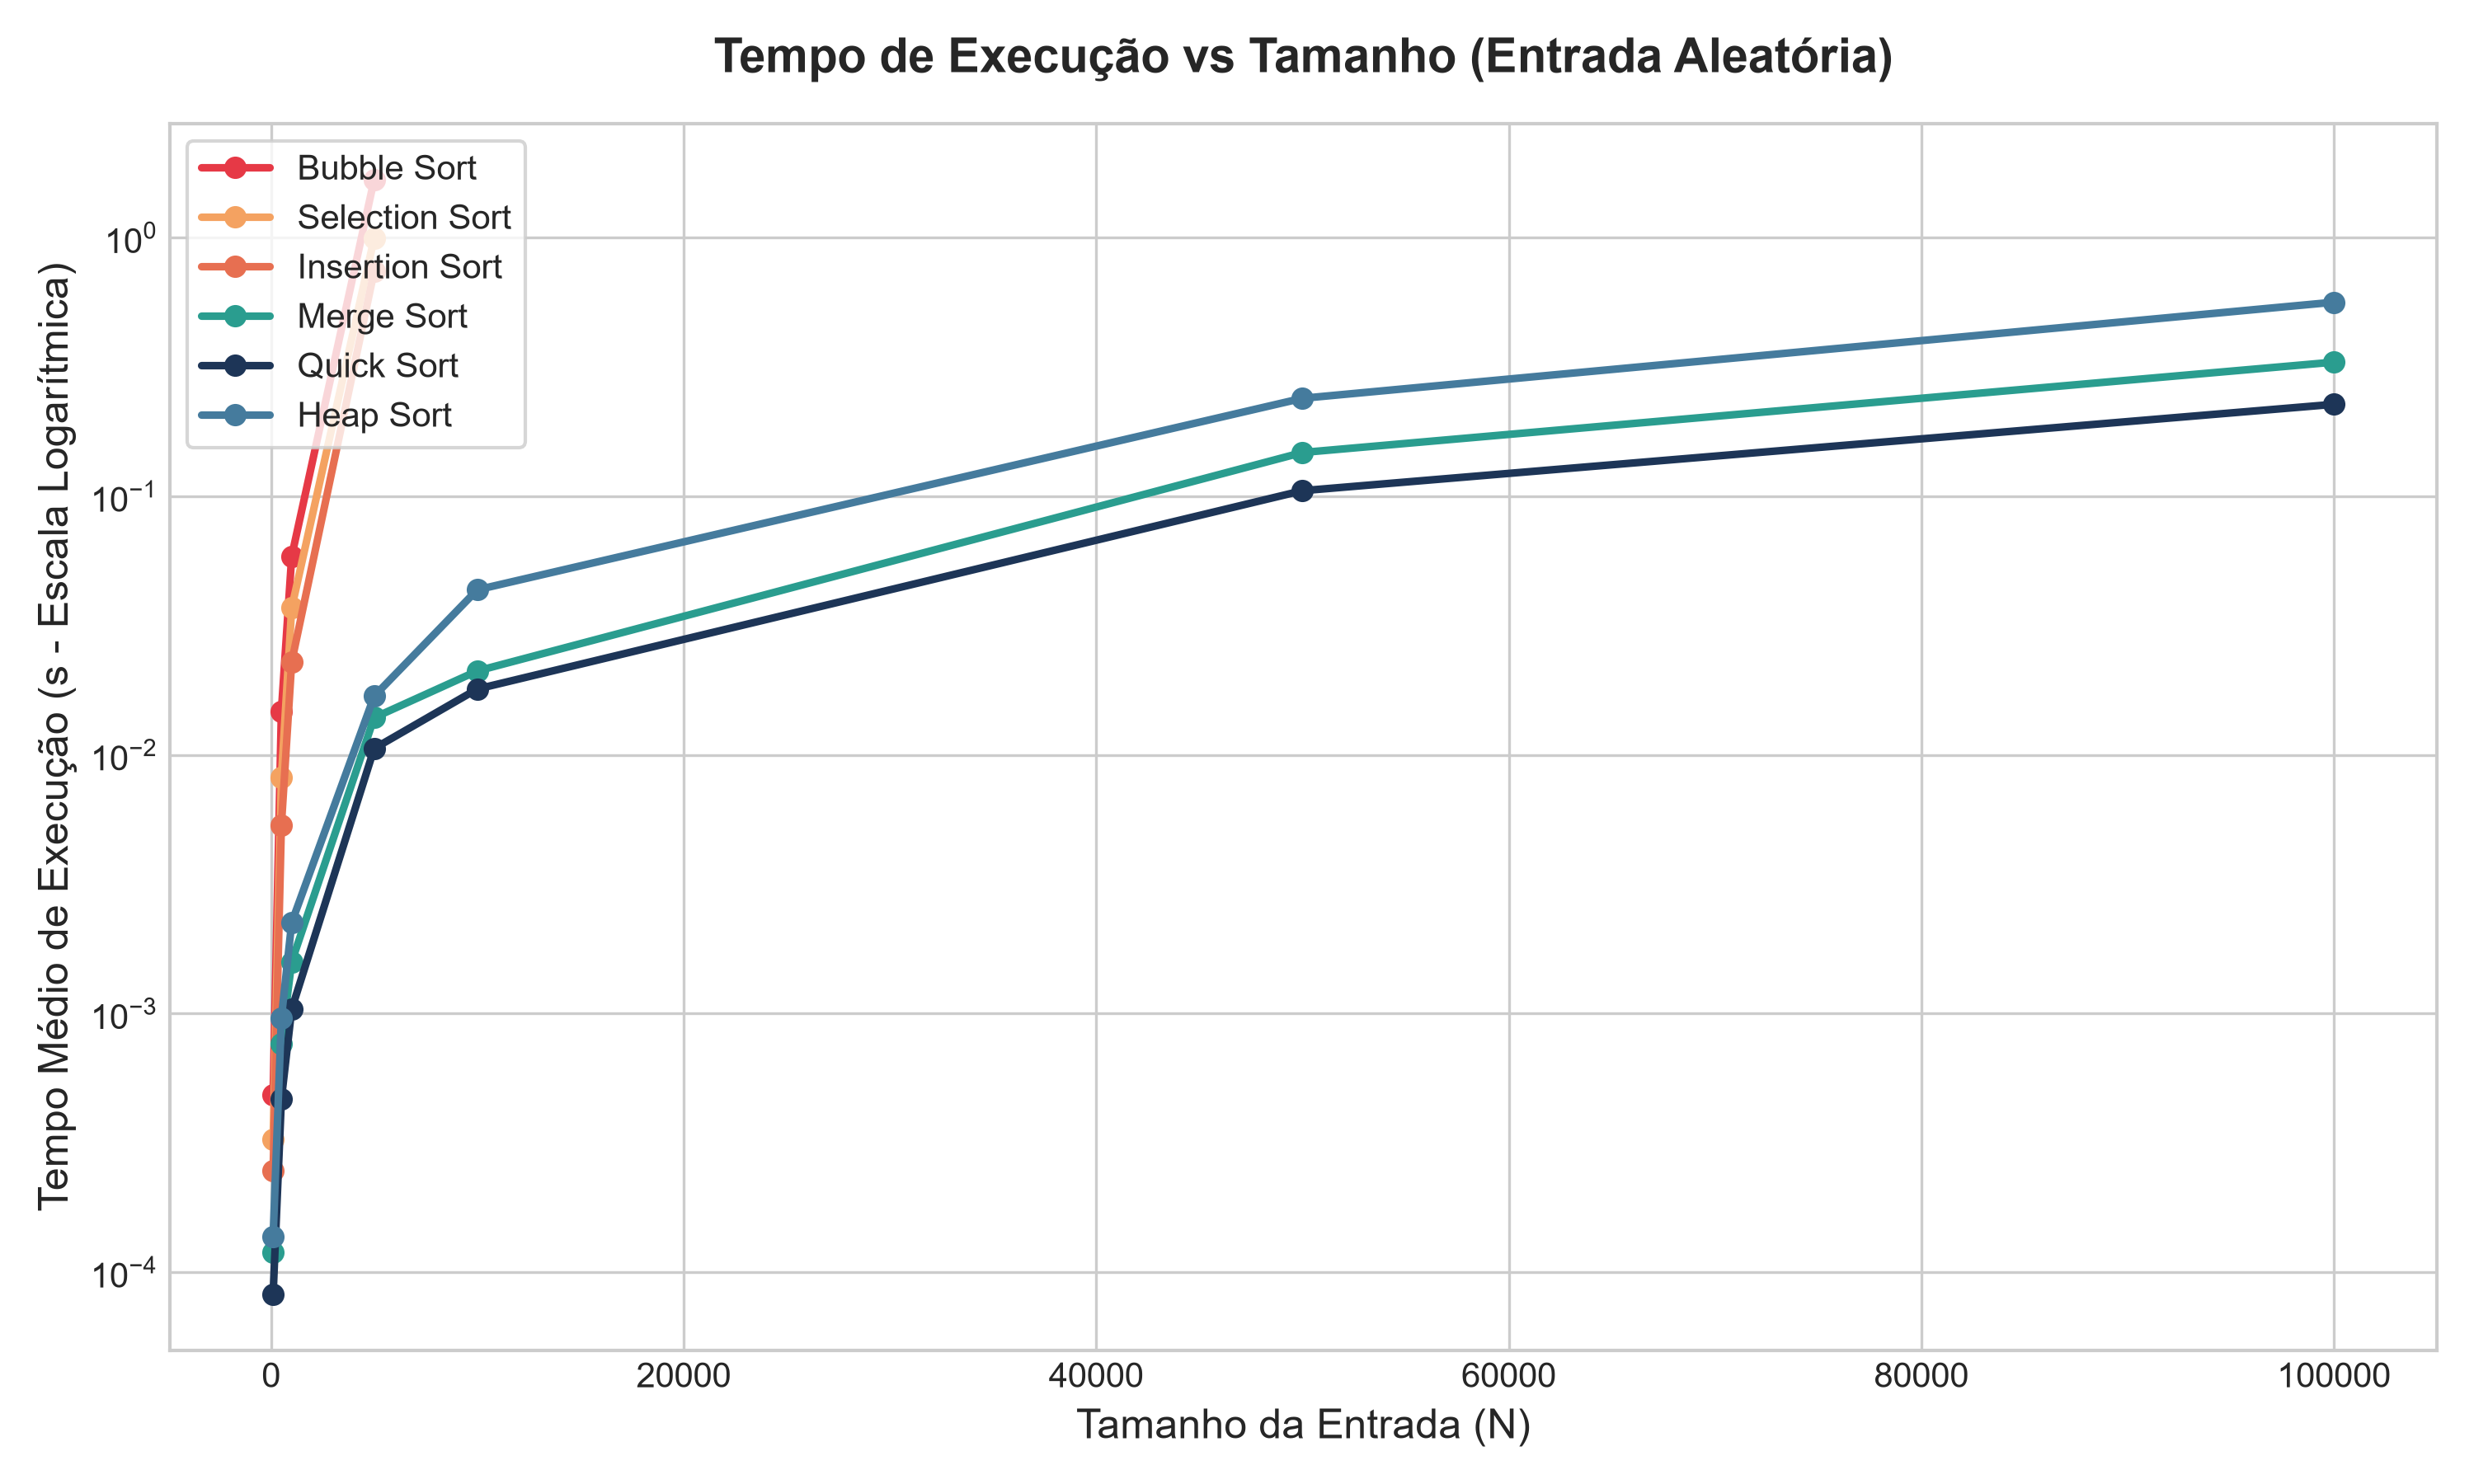
\includegraphics[width=0.75\textwidth]{../bench/charts/time_comparison_random.png}
    \end{center}
\end{frame}

\begin{frame}{Comparativo Direto ($N = 5.000$ Elementos)}
    \begin{center}
        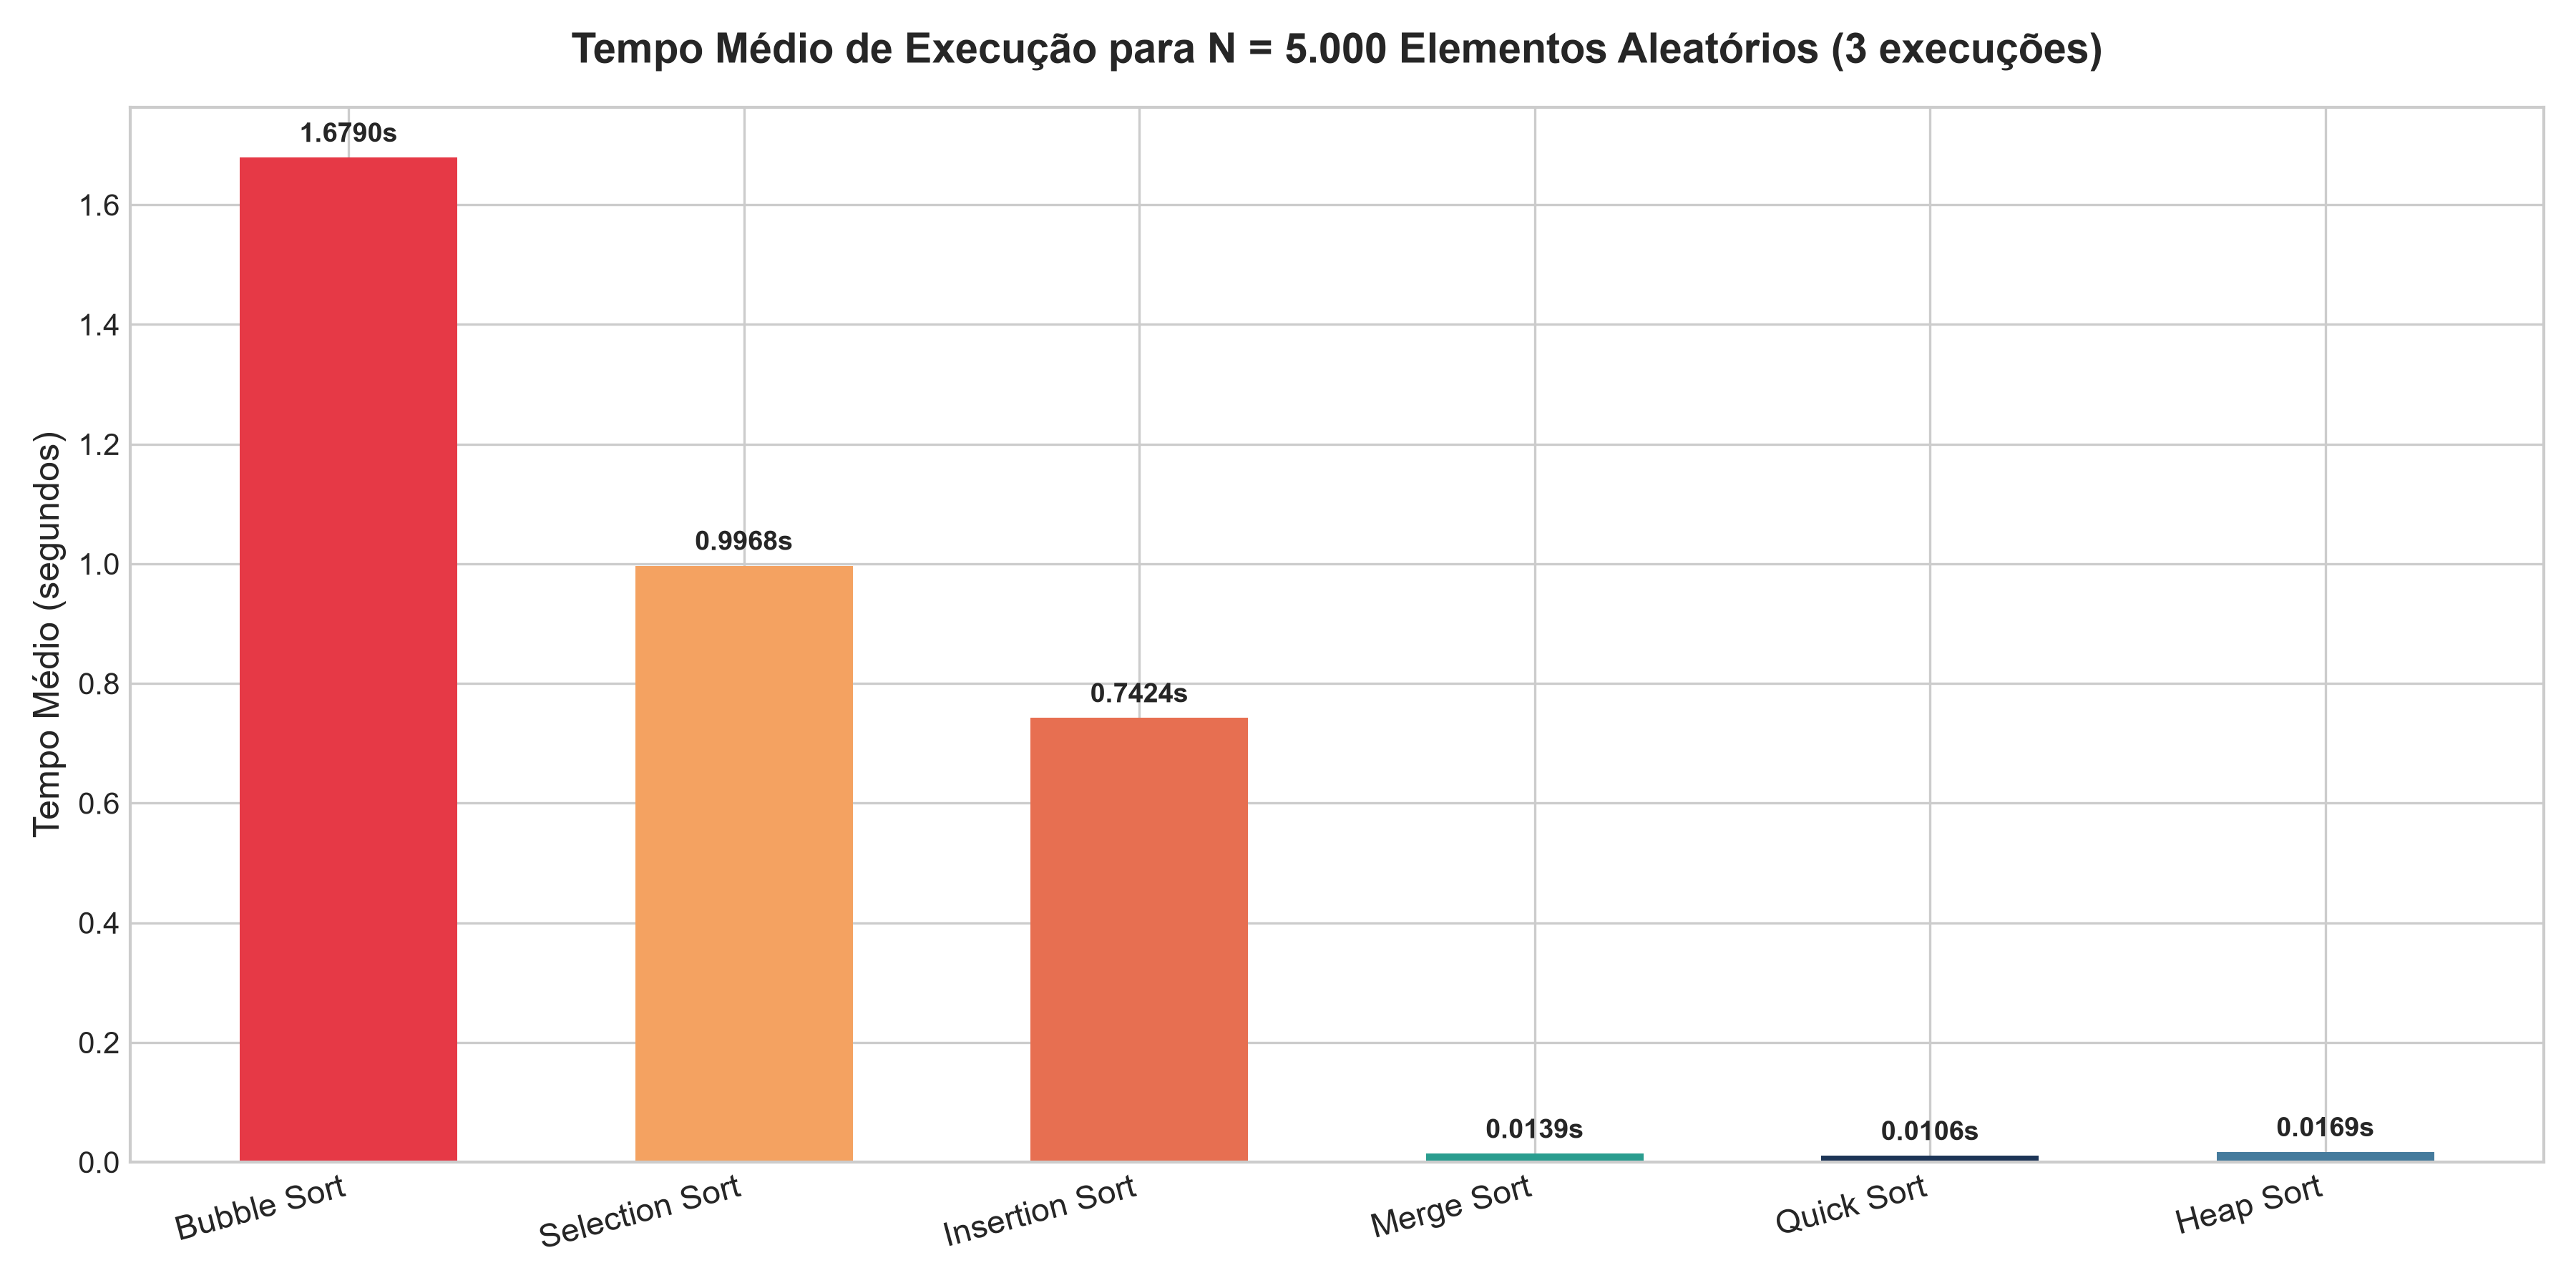
\includegraphics[width=0.75\textwidth]{../bench/charts/overall_comparison_bar.png}
    \end{center}
\end{frame}

\begin{frame}{Entrada Quase Ordenada (5\% de permutações)}
    \begin{center}
        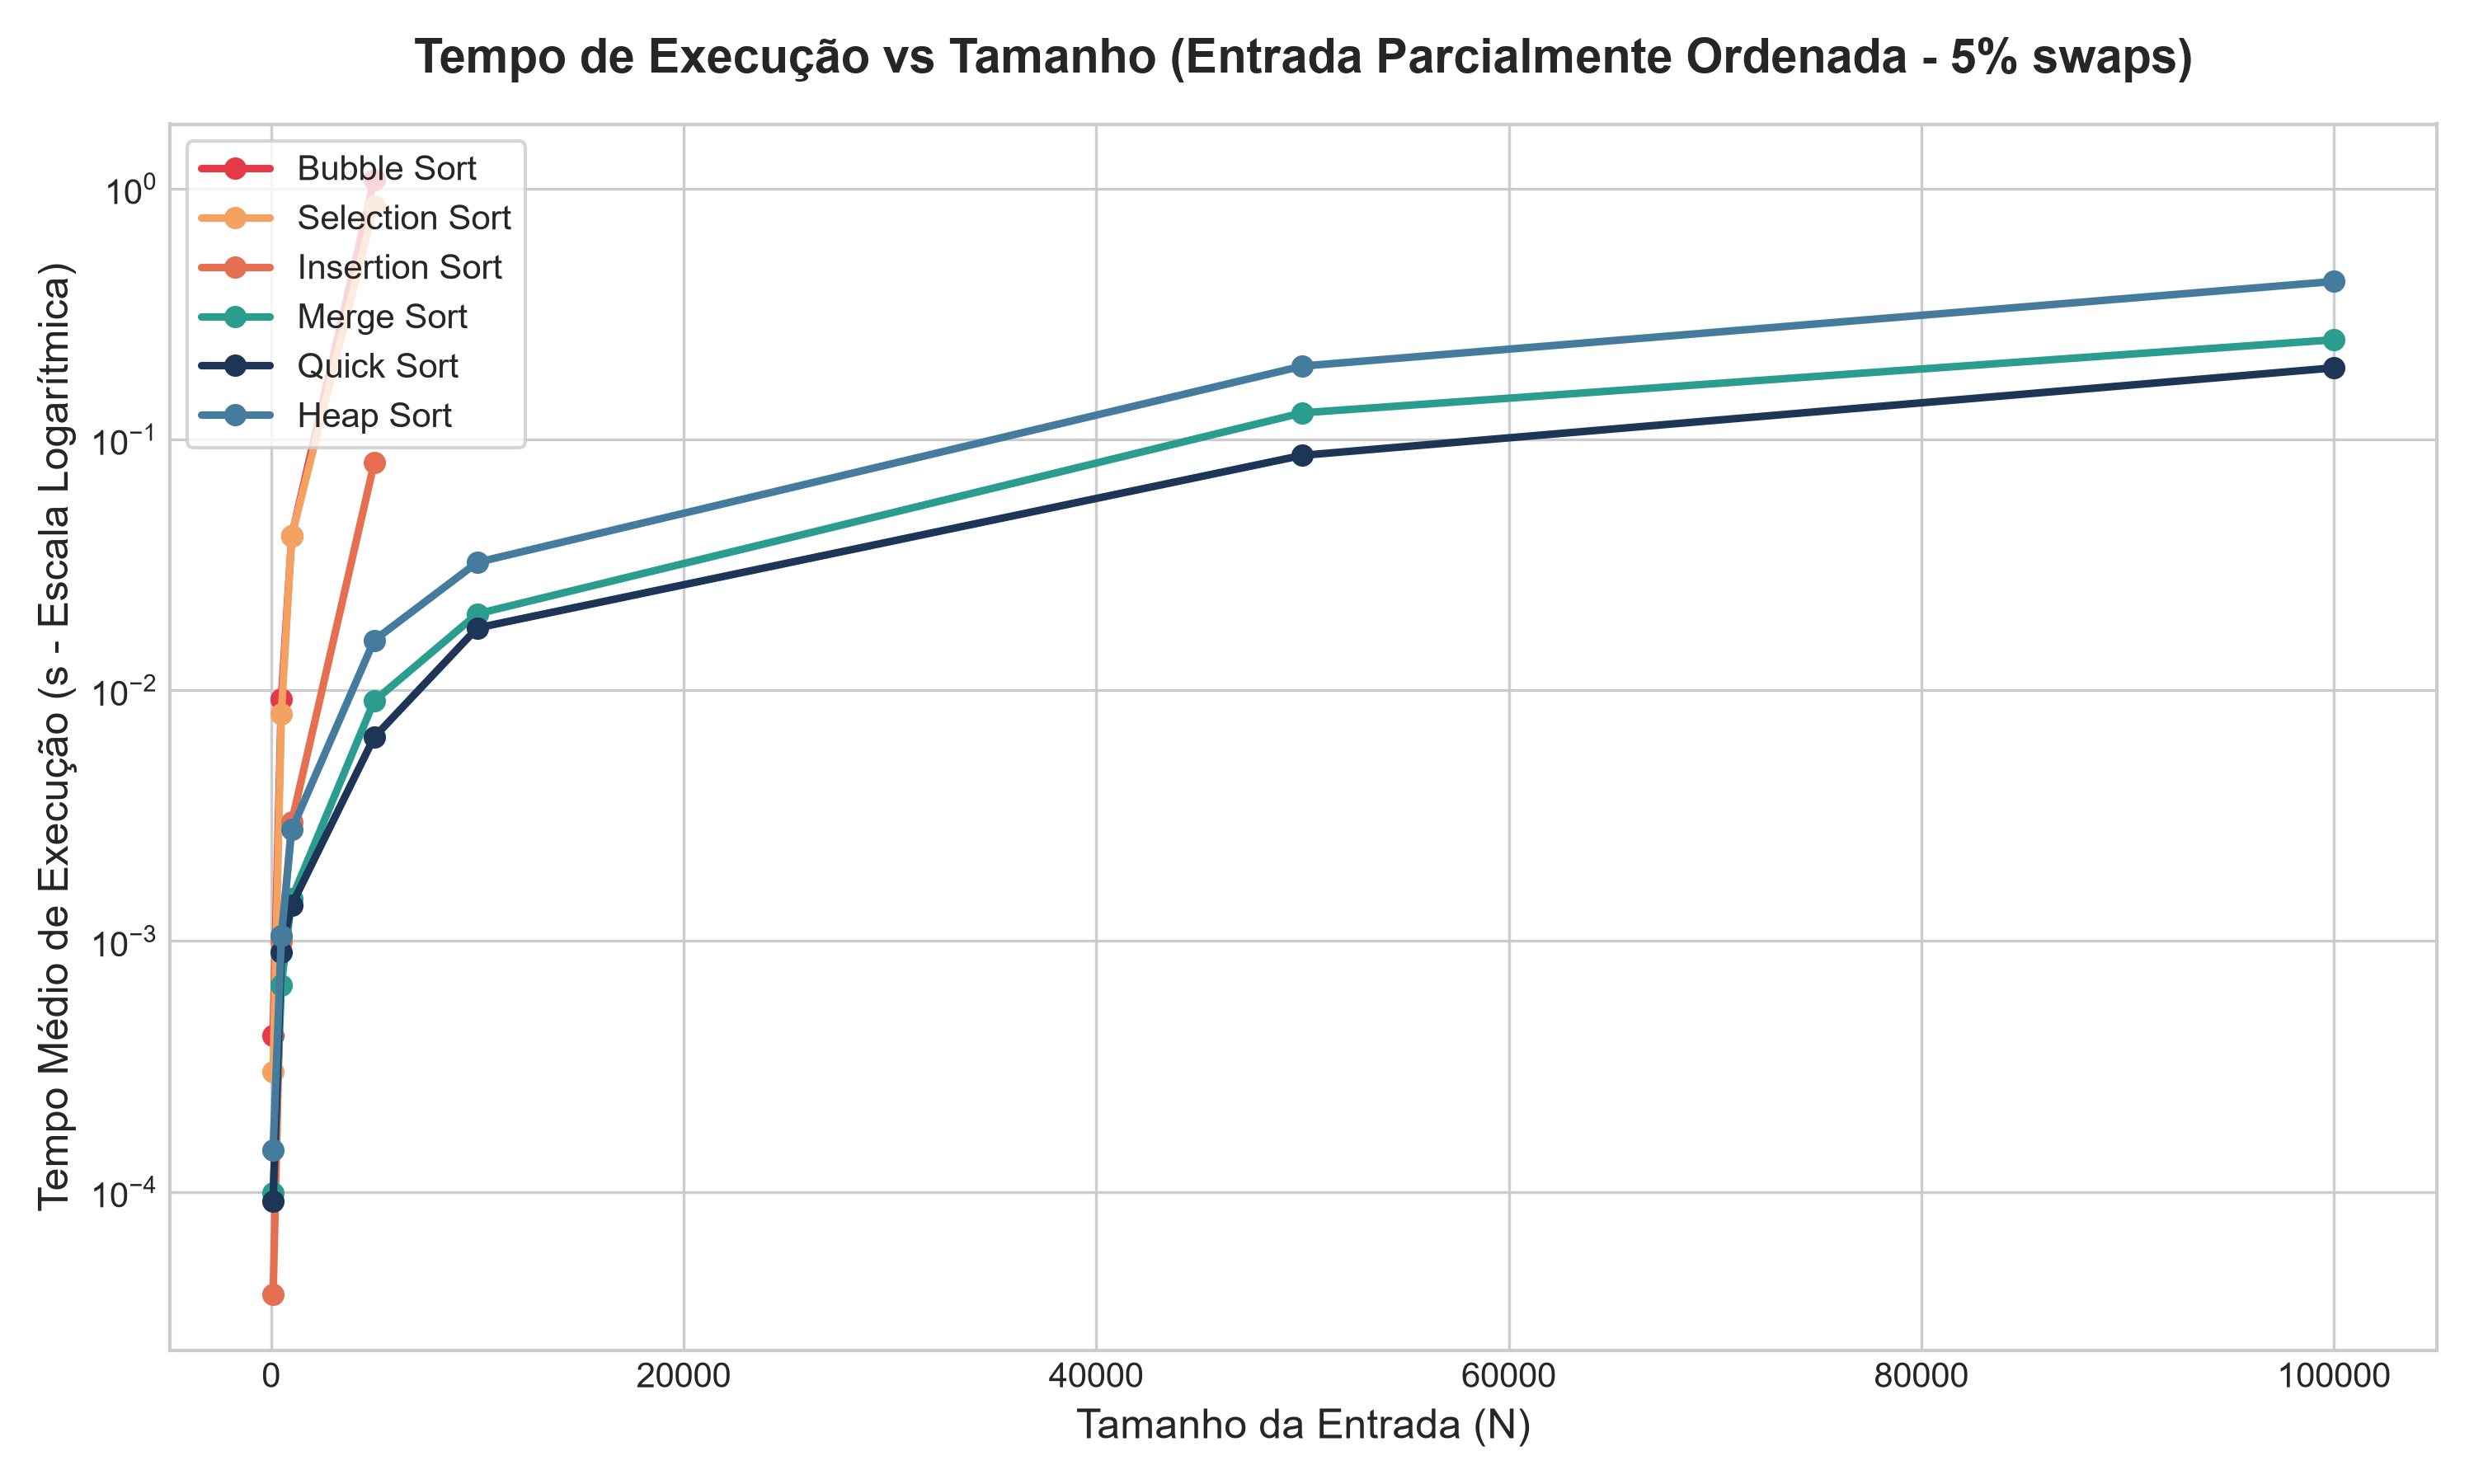
\includegraphics[width=0.75\textwidth]{../bench/charts/time_comparison_nearly_sorted.png}
    \end{center}
    \small \textbf{Destaque:} Insertion Sort atinge desempenho quase linear ($O(n)$) superando algoritmos $O(n \log n)$.
\end{frame}

\begin{frame}{Objetos Customizados vs Tipos Primitivos}
    \begin{center}
        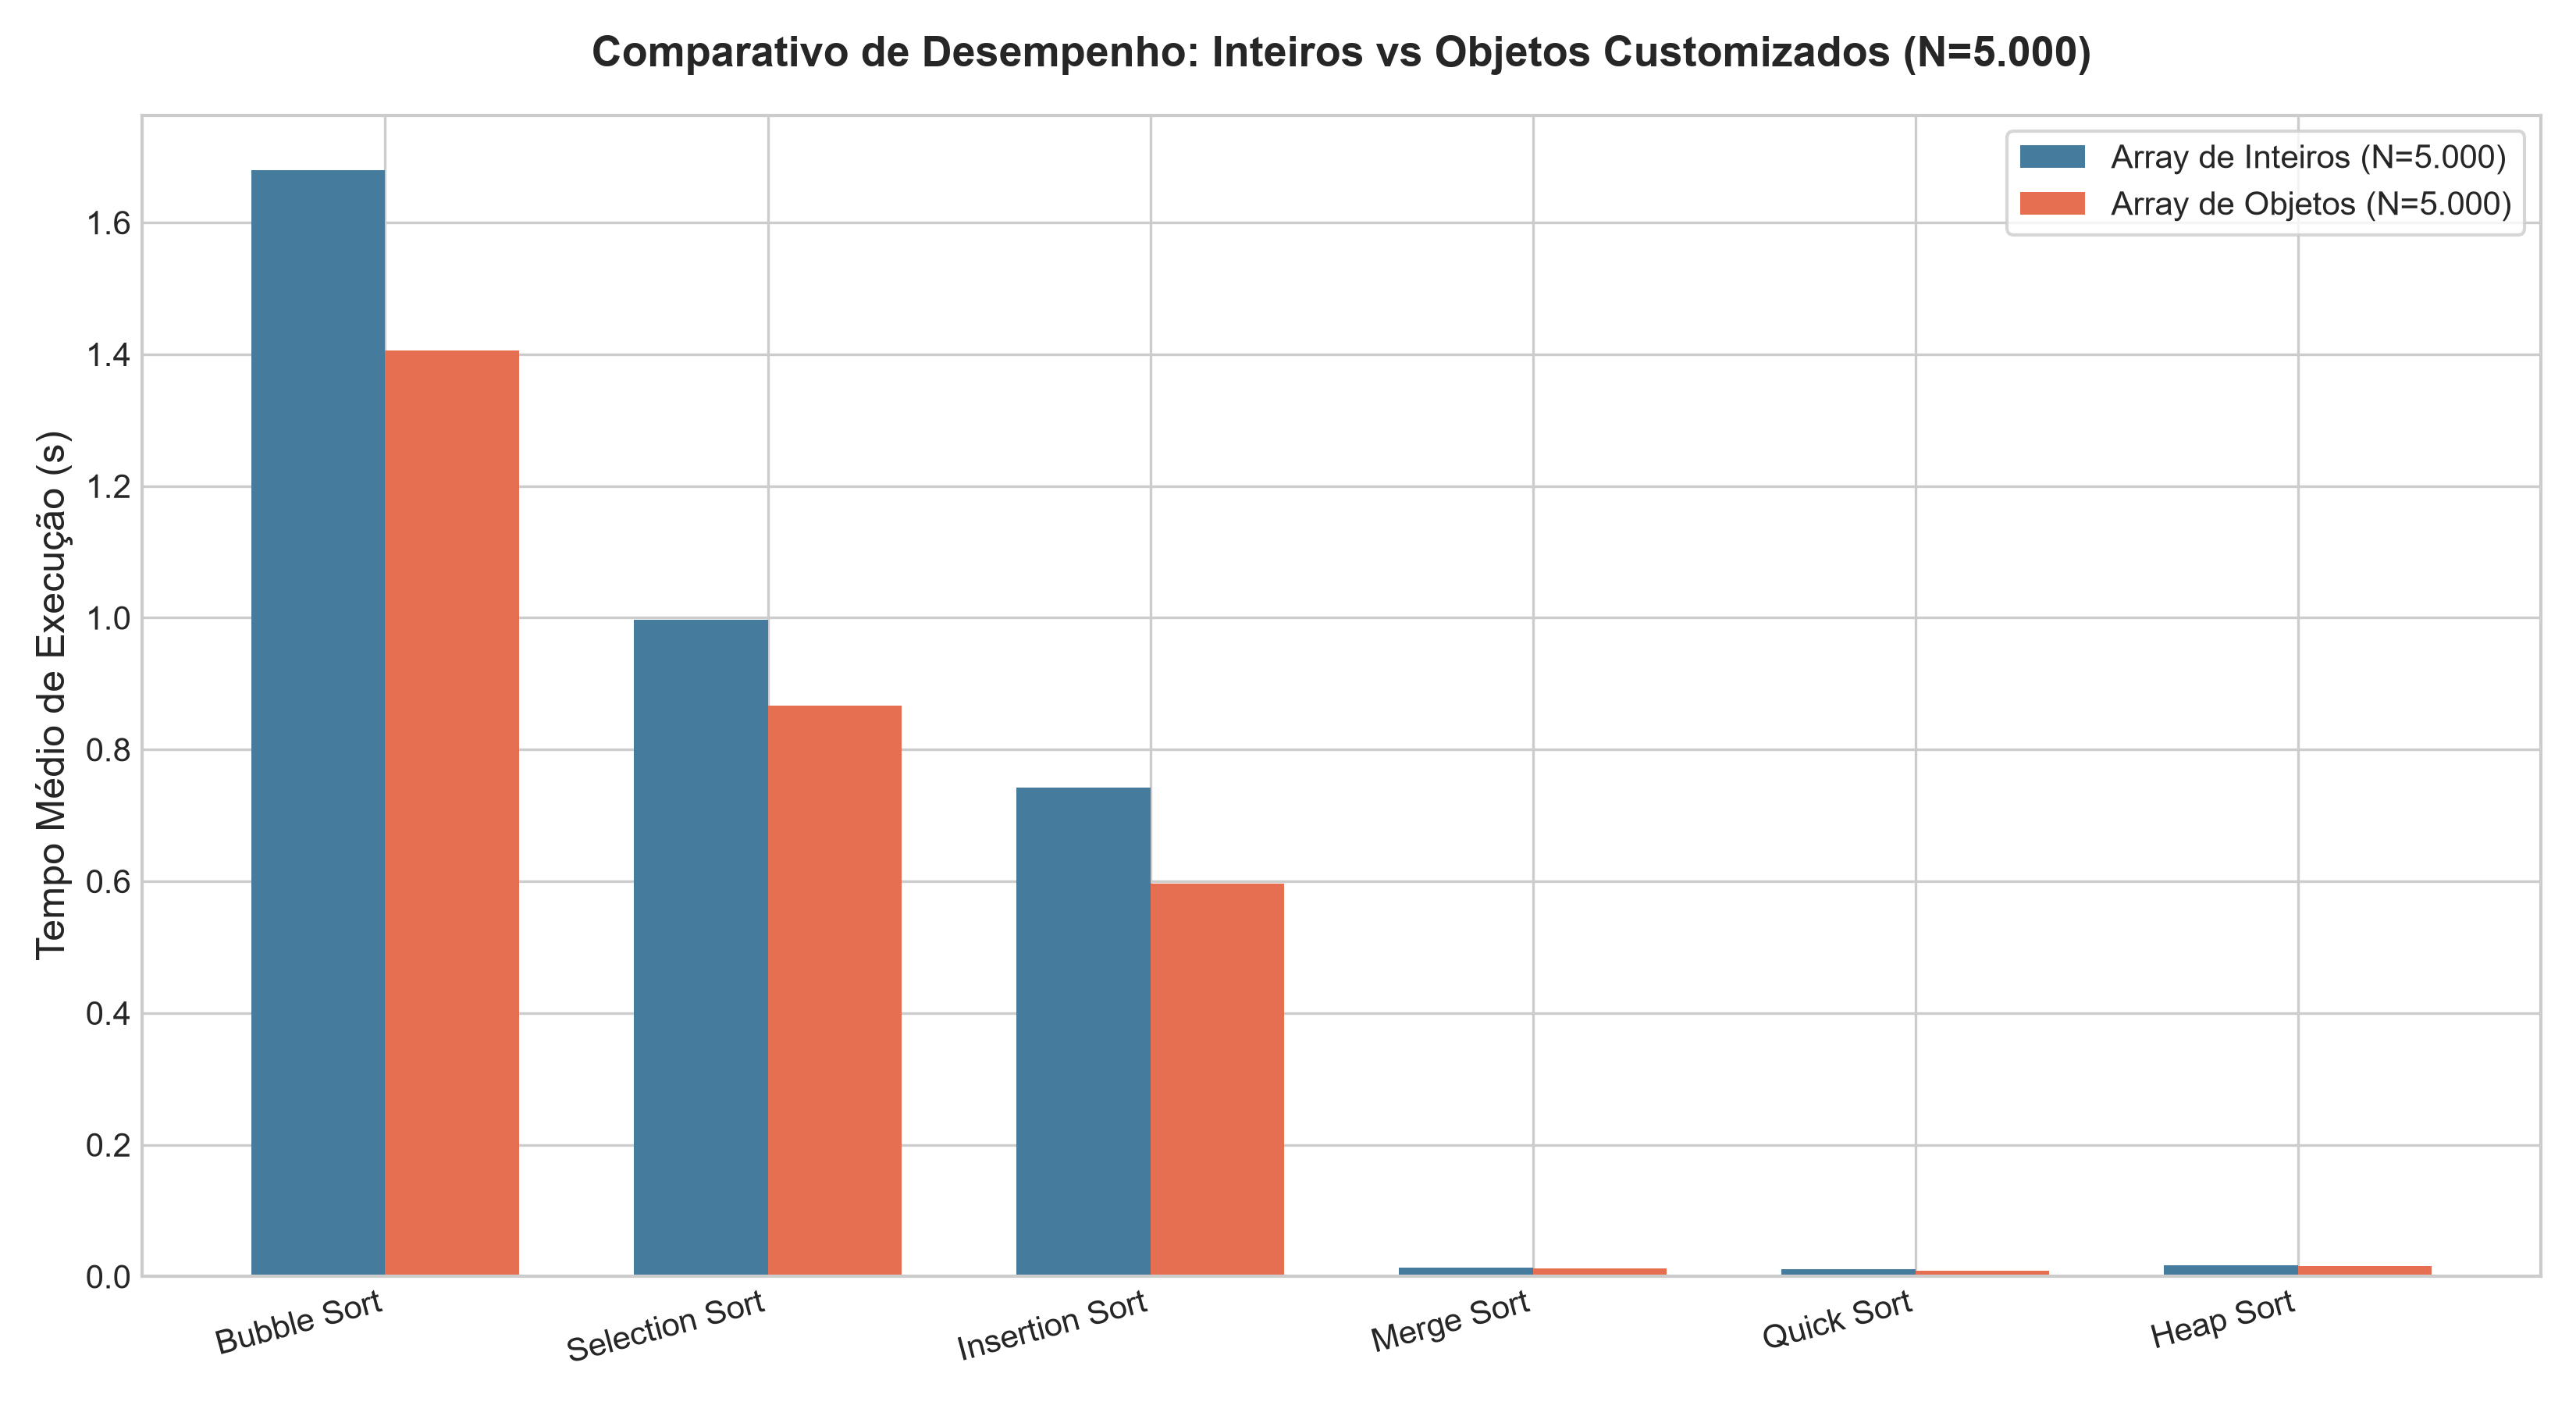
\includegraphics[width=0.75\textwidth]{../bench/charts/primitives_vs_objects.png}
    \end{center}
    \small A sobrecarga de extração de chave afeta proporcionalmente mais algoritmos com elevado número de comparações.
\end{frame}

\section{Conclusões e Recomendações}
\begin{frame}{Recomendações Práticas}
    \begin{itemize}
        \item \textbf{Dados Aleatórios Gerais ($N > 1.000$):} Quick Sort é o mais rápido (eficiência de cache e baixa constante).
        \item \textbf{Dados Quase Ordenados ou $N < 50$:} Insertion Sort é o ideal.
        \item \textbf{Estabilidade Mandatória:} Merge Sort.
        \item \textbf{Memória Crítica $O(1)$ sem pior caso quadrático:} Heap Sort.
    \end{itemize}
\end{frame}

\begin{frame}
    \begin{center}
        \Huge \textbf{Obrigado!} \\
        \vspace{0.5cm}
        \Large Perguntas?
    \end{center}
\end{frame}

\end{document}
